\documentclass[mathserif]{beamer}

\usepackage[utf8]{inputenc}    % enables use of utf8 characters in the input file
\usepackage[T1]{fontenc}       % enables proper output of unicode characters such that text can be copy-pasted from the pdf file
\usepackage{times}             % replaces Computer Modern font with something resembling Times
\usepackage{graphicx}          % enables including graphics
\usepackage{amsmath}           % ams math module
\usepackage{amssymb}           % ams math symbols
\usepackage{mathtools}         % fixes a few quirks with the ams packages

% functions
\DeclareMathOperator{\atan2}{atan2}
\DeclareMathOperator*{\argmin}{argmin}
\DeclareMathOperator*{\argmax}{argmax}

% braces
\newcommand{\xp}[1]{\left(#1\right)}   % parentheses
\newcommand{\xb}[1]{\left[#1\right]}   % brackets
\newcommand{\xc}[1]{\left\{#1\right\}} % curly braces
\newcommand{\xa}[1]{\left|#1\right|}   % absolute value
\newcommand{\xn}[1]{\left\|#1\right\|} % vector norm

% types
\newcommand{\function}[2]{#1 \rightarrow #2}
\newcommand{\R}[1]{\mathbb{R}^{#1}}
\newcommand{\RR}{\mathbb{R}}
\newcommand{\unit}{\xb{0,1}}

% complex terms
\newcommand{\apply}[2]{#1\!\xp{#2}}
\newcommand{\integral}[4]{\int_{#1}^{#2} #3 \; \mathrm{d}#4}
\newcommand{\powerset}[1]{\apply{\mathcal{P}}{#1}}

% continuity
\newcommand{\contp}[1]{\mathrm{C}^{#1}}
\newcommand{\contg}[1]{\mathrm{G}^{#1}}

% vectors
\newcommand{\vectorA}[1]{\begin{pmatrix}#1\end{pmatrix}}
\newcommand{\vectorB}[2]{\begin{pmatrix}#1\\\linebreak{}#2\end{pmatrix}}
\newcommand{\vectorC}[3]{\begin{pmatrix}#1\\\linebreak{}#2\\\linebreak{}#3\end{pmatrix}}
     % some math helper macros

\useoutertheme[subsection=false]{miniframes}
\useinnertheme{default}
\usecolortheme{default}
\setbeamertemplate{navigation symbols}

\title{Optimal Fitting of Planar Curves to Prescribed Constraints}
\author{Julian Asamer, Julian Brunner}
\date{\today}

\begin{document}

	\begin{frame}
		\titlepage
	\end{frame}

	\section{Introduction}

		% A
		\begin{frame}
			\frametitle{Introduction}
			\begin{itemize}
				%illustrations, cartoons, industrial design
				\item vector graphics are widely used
				\item 2D vector graphics primitives are curves
				\item design process of curves is very important
				\item designing curves with current tools can be frustrating
				% artist has a hard time to make the curve look the way he wants to
				% often unclear why
				% it's hard to communicate intentions
				\item research has been done in different directions with little impact
				\item our objective: improved curve design process
				% identify nature and cause of shortcomings in current curve design tools 
				% develop a better curve design tool
			\end{itemize}
		\end{frame}
		
	\section{Problem Analysis}

		% A
		\begin{frame}
			\frametitle{The Curve Design Process}
			\begin{itemize}
				\item obtain source curve
				% as real or mental image, obviously software-independent
				\item extract properties from the source curve 
				\item provide them to the software
				% strongly dependent on curve design tool - the software dictates which properties can be entered
				\item the software constructs a curve
				% if the curve is not precisely specified, a fairness measure is used to derive the most likely result curve
				% iteration over steps 2-4 to adjust the curve until satisfactory alignment with the source curve is reached
			\end{itemize}
		\end{frame}

		% A
		\begin{frame}
			\frametitle{Usability Criteria for Curve Design Tools}
			\begin{itemize}
				% specification language determines the properties of a curve that can be specified
				% such properties or specifications are fullfilled by a potentially infinite number of curves
				% fairness measure selects one curve
				% curve design tools can affect the design process by choosing specification language and fairness measure, and practical ability to derive curves from them
				\item description language := specification language + fairness measure
				\item specification language should be
				\begin{itemize}
					\item expressive
					% easy to handle for humans
					\item easy
					% allow efficient communication of intent
					\item efficient
				\end{itemize}
				\item fairness measure should
				\begin{itemize}
					% capture intuitive notions of smoothness
					\item ensure smoothness
					% select curves that are minimal in respect to the specification
					\item select minimal curves
				\end{itemize}
				\item ability to derive curves from descriptions
			\end{itemize}
		\end{frame}

		% B	
		\begin{frame}
			\frametitle{Bézier Splines}
			\begin{itemize}
				\item most popular curve type
				\item specify point and velocity at start and end of each segment
				\item fairness measure `chooses' unique cubic polynomial
				\item most usability criteria fulfilled sufficiently
				\item usability problems
				\begin{itemize}
					\item curvature continuity is not guaranteed
					% hard to choose coefficient points in a way that results in curvature continuity
					% software support for curvature continuity sacrifices degrees of freedom
					\item lack of expressiveness of the specification language
					% curvature cannot be specified directly
					% hard to get constant/linearly changing curvature ==> circular arcs/spirals are hard to specify
					% high number of segments sacrifices smoothness
				\end{itemize}
			\end{itemize}
		\end{frame}

		% B
		\begin{frame}
			\frametitle{Bézier Splines - Examples}
			\center{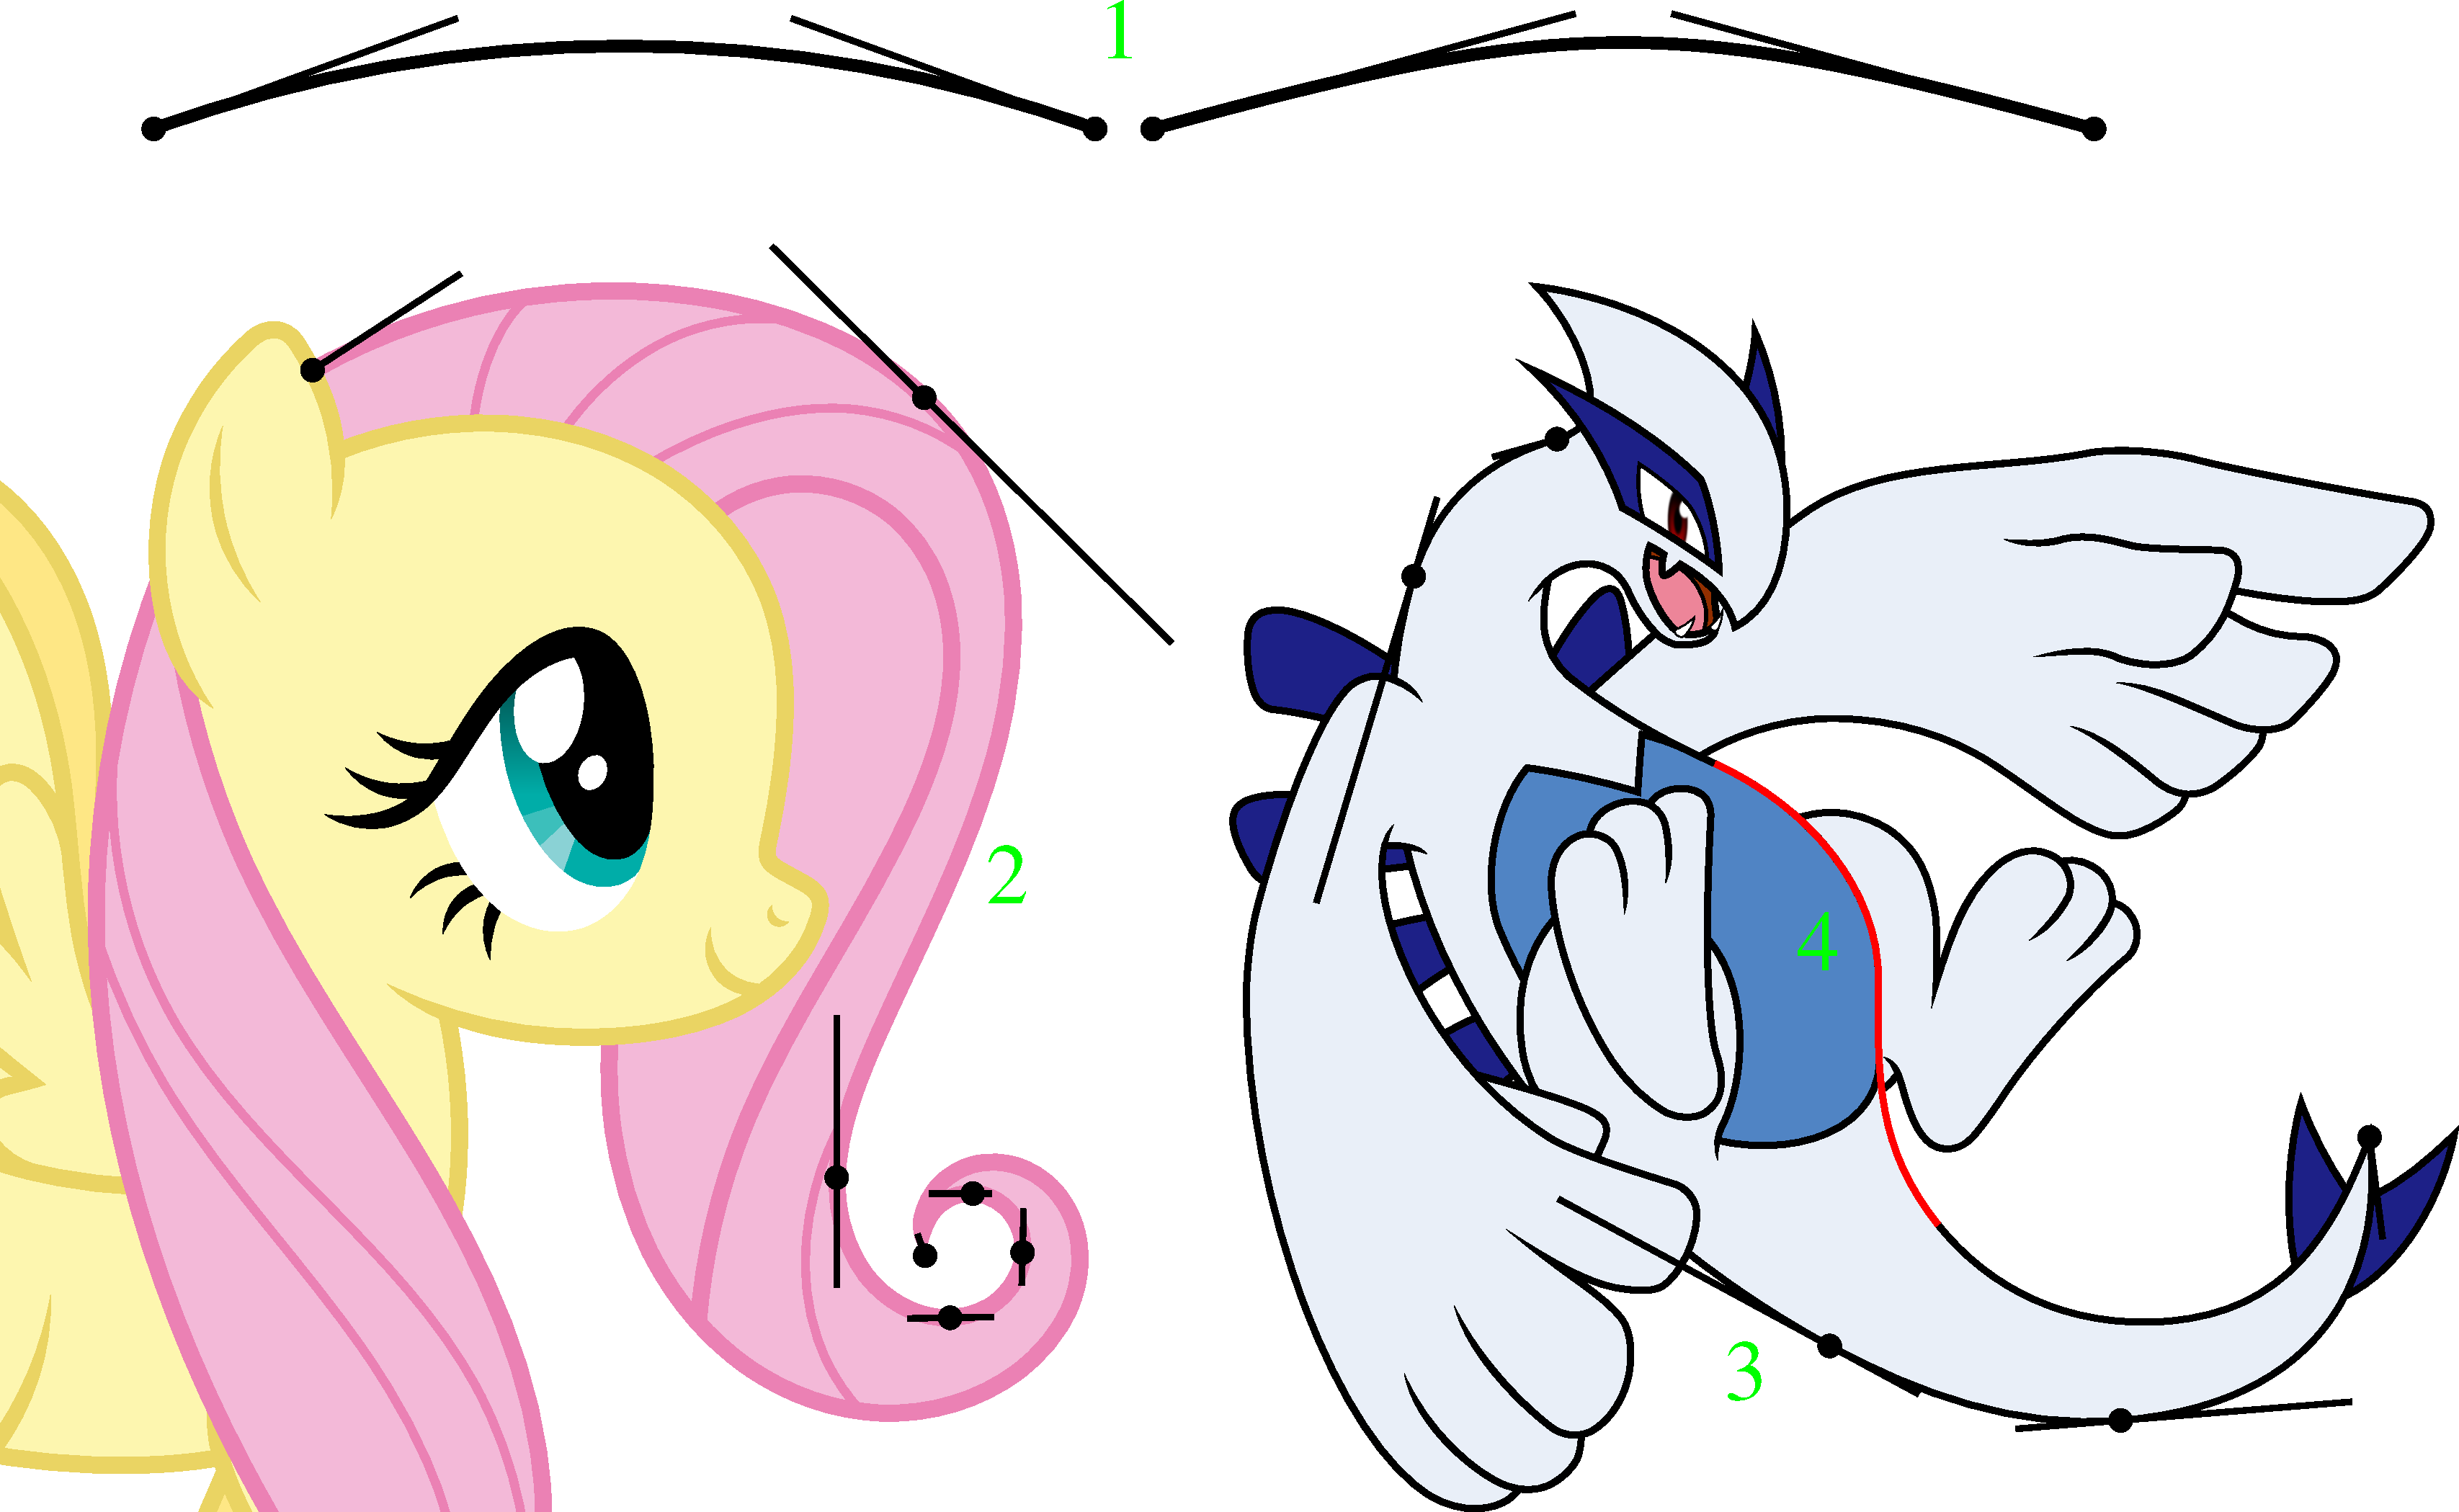
\includegraphics[width=\textwidth]{../resources/usability_bezier.pdf}}\\
			% nodes: red dots, handles: green tangent lines
			% 1: circular arc
			%   difference hard to see, frequent mistakes when doing circular arcs
			% 2, 3: curves better described using curvature
			%   2: many nodes, decreased smoothness
			%   3: hard to modify
			% 4: curvature discontinuity
			%   upper part constant curvatur, lower part goes to zero curvature
			%   would be even harder to spot if line wasn't vertical
		\end{frame}

		% B
		\begin{frame}
			\frametitle{Spiro Splines}
			\begin{itemize}
				\item consist of parts of the Euler spiral
				% Euler spiral: curvature changes linearly with arc length
				\item construct interpolating splines
				% can only specify points, no direction, no curvature
				\item fairness measure guarantees curvature continuity
				\item usability problem: lack of expressiveness of the specification language
				% direction and curvature need to be specified indirectly (same problems as with Bézier splines)
				% unfortunate: Euler spiral segments perfect for constant/linearly changing curvature
			\end{itemize}
		\end{frame}

		% B
		\begin{frame}
			\frametitle{Spiro Splines - Examples}
			\center{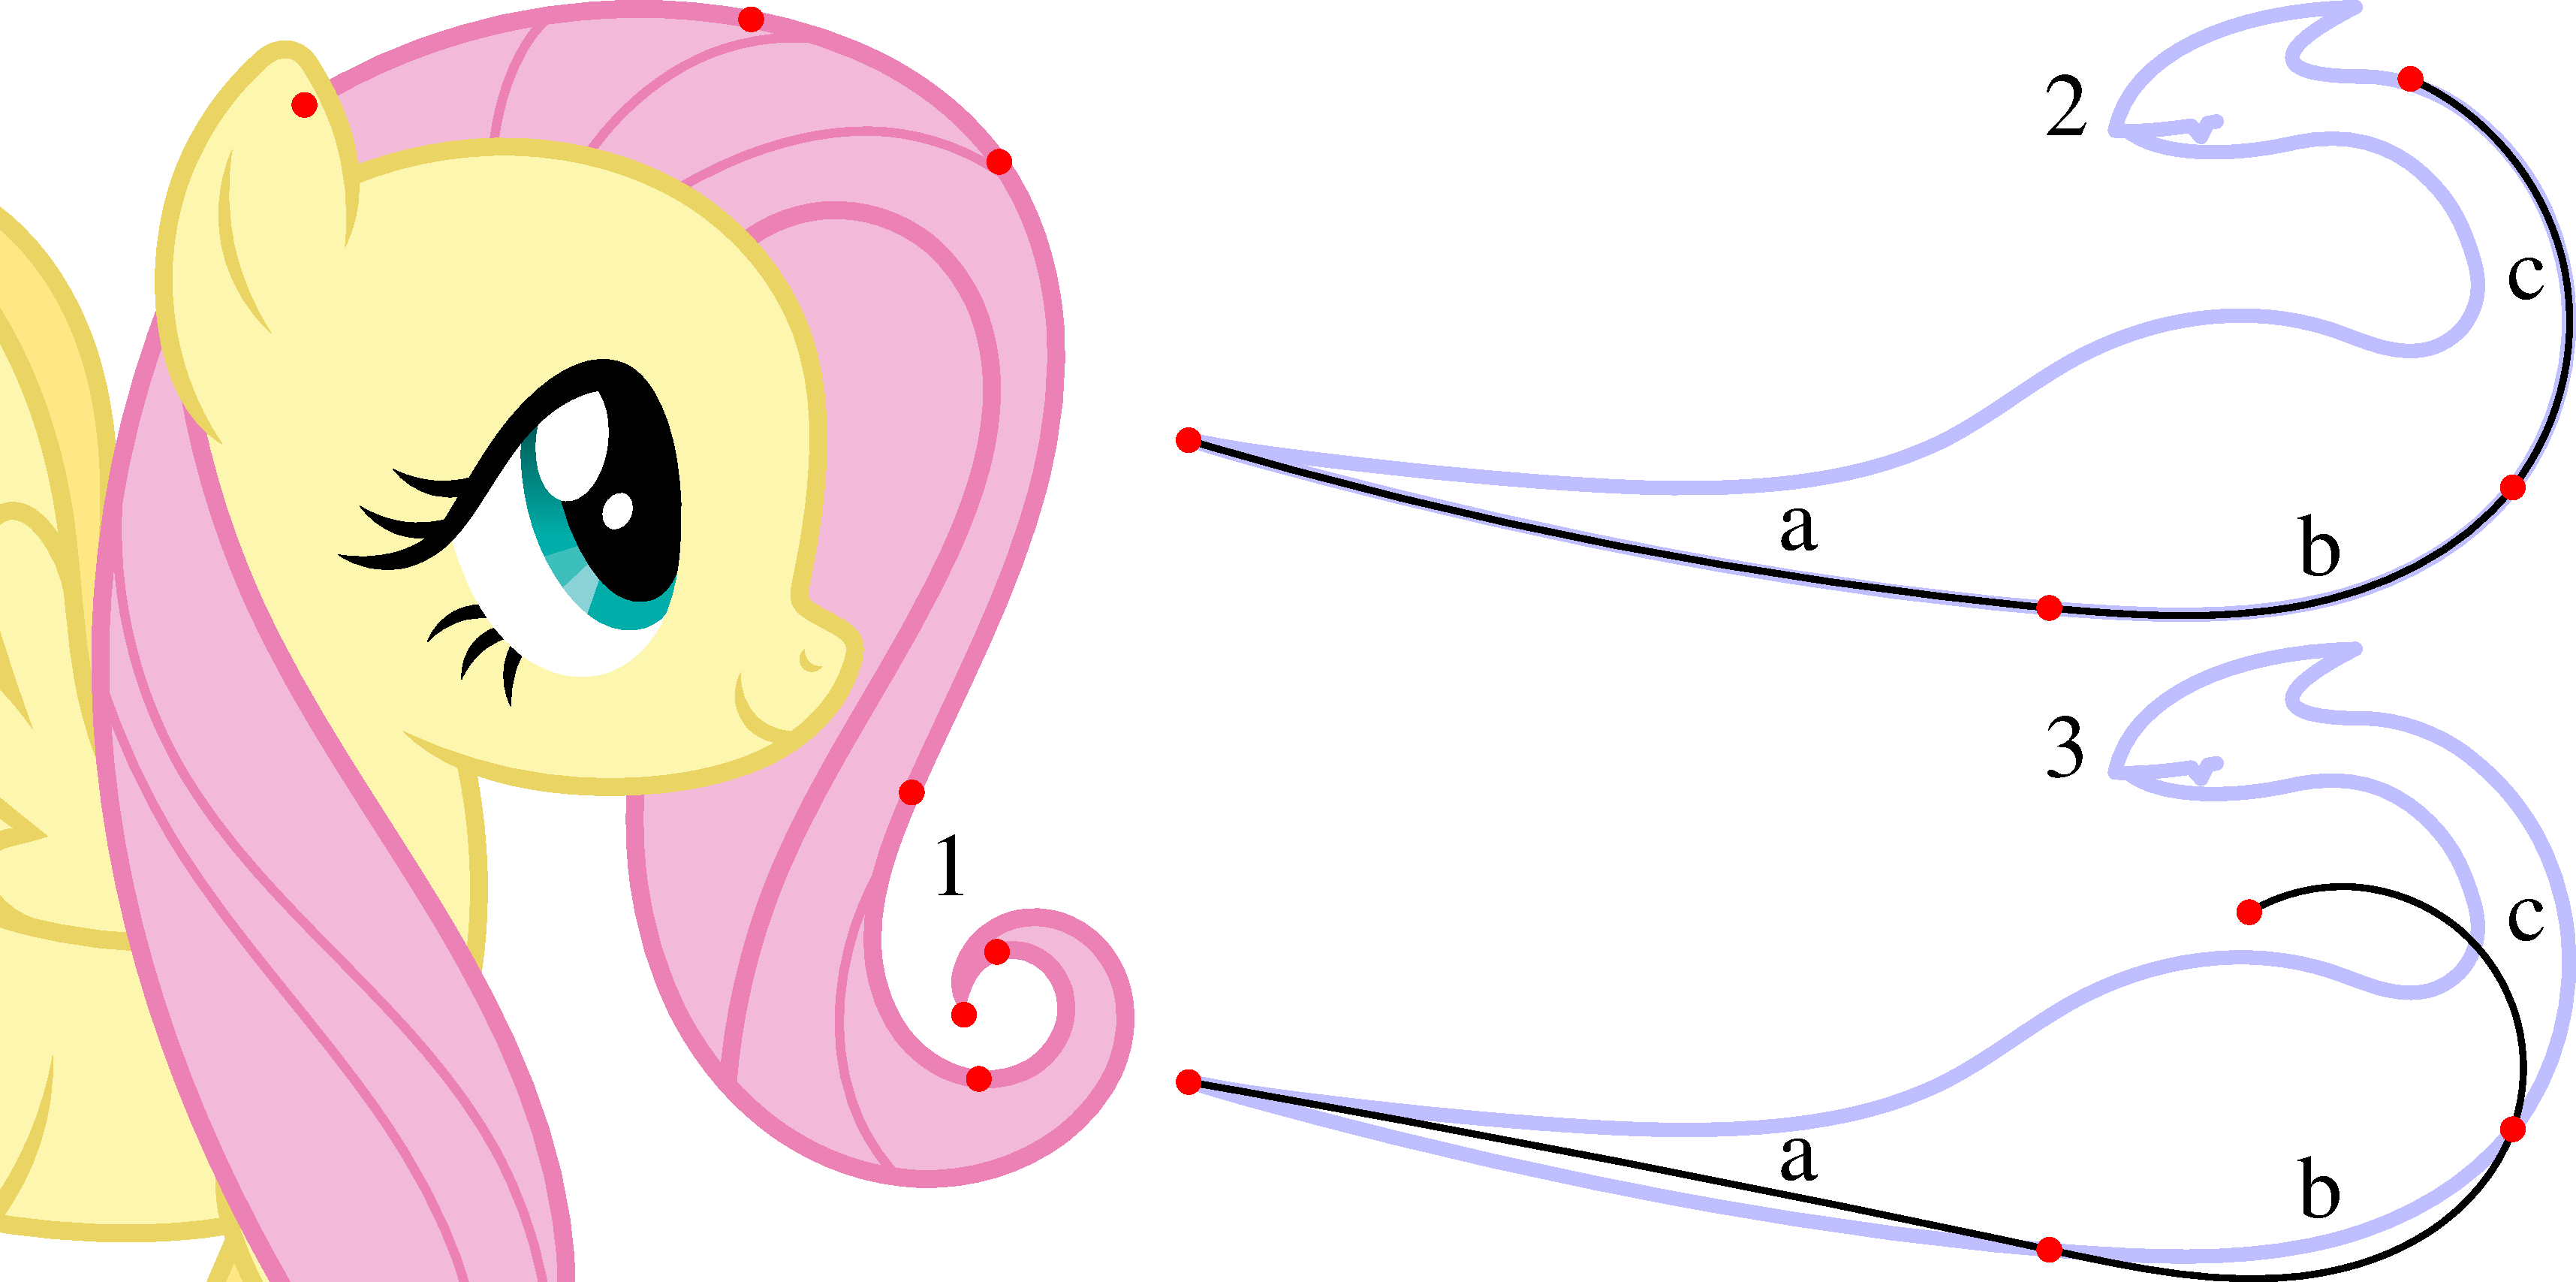
\includegraphics[width=\textwidth]{../resources/usability_spiro.pdf}}\\
			% control points: red dots
			% 1: spiral
			%   well-suited for parts of Euler spiral
			%   many control points with Spiro spline, still less than with Bézier Spline (about 1/3 of the information)
			% 2: few carefully placed control points
			%   low curvature, linear change, high curvature
			%   only 4 control points
			% 3: bad handling of modifications
			%   indirectly increase curvature in segment c by moving control point
			%   curvature in segment a is affected, relied on fragile configuration
		\end{frame}
	
	\section{Proposed Solution}

		% A
		\begin{frame}
			\frametitle{Definitions}
			\begin{align*}
				\phi    & : \function{\unit}{\R{2}} && \text{point}\\
				\sigma  & : \function{\unit}{\RR}   && \text{speed}\\
				\lambda & : \function{\unit}{\RR}   && \text{covered arc length}\\
				\delta  & : \function{\unit}{\RR}   && \text{direction}\\
				\chi    & : \function{\unit}{\RR}   && \text{curvature}
			\end{align*}
		\end{frame}

		% A
		\begin{frame}
			\frametitle{Description-Based Curves - Motivation}
			\begin{itemize}
				\item description language has huge effect on usability
				\item should not be based on low-level mathematical aspects % beziér
				\item do not impose limitations on specification language prematurely % spiro
				\item we need a good specification language and fairness measure
			\end{itemize}
		\end{frame}

		% A
		\begin{frame}
			\frametitle{Description-Based Curves}
			\center{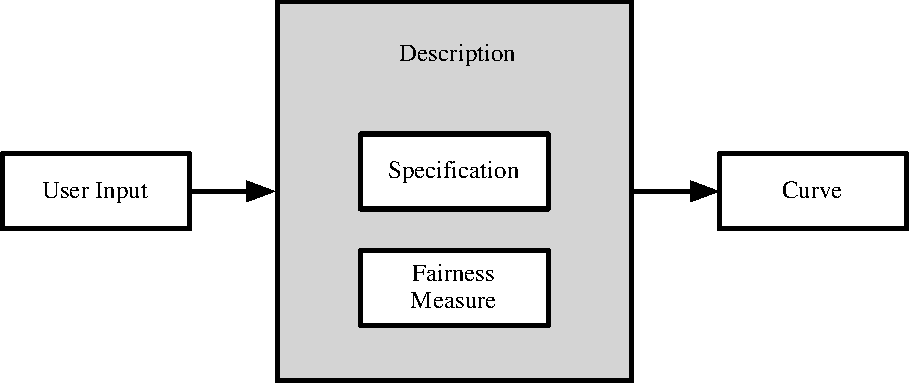
\includegraphics[width=\textwidth]{../resources/description-based_curves.pdf}}\\
		\end{frame}

		% A
		\begin{frame}
			\frametitle{Specification Language}
			% contains all the reasoning about the specification language
			\begin{itemize}
				\item decoupled from underlying curve model
				\item allows specification of geometric properties
				\item point, direction, curvature
				\item any combination, any position
				\item positioning via fraction of arc length of curve
				\item total curve length specified as well
			\end{itemize}
		\end{frame}

		% A
		\begin{frame}
			\frametitle{Specification Language - Example}
			\center{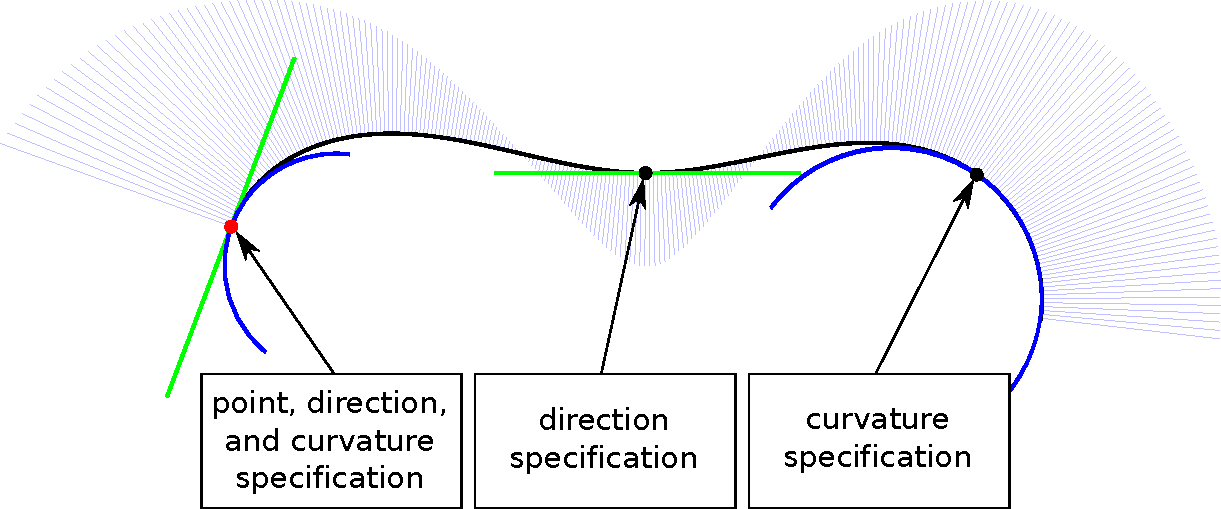
\includegraphics[width=\textwidth]{../resources/specification_example.pdf}}\\
		\end{frame}

		% A
		\begin{frame}
			\frametitle{Fairness Measure}
			\center{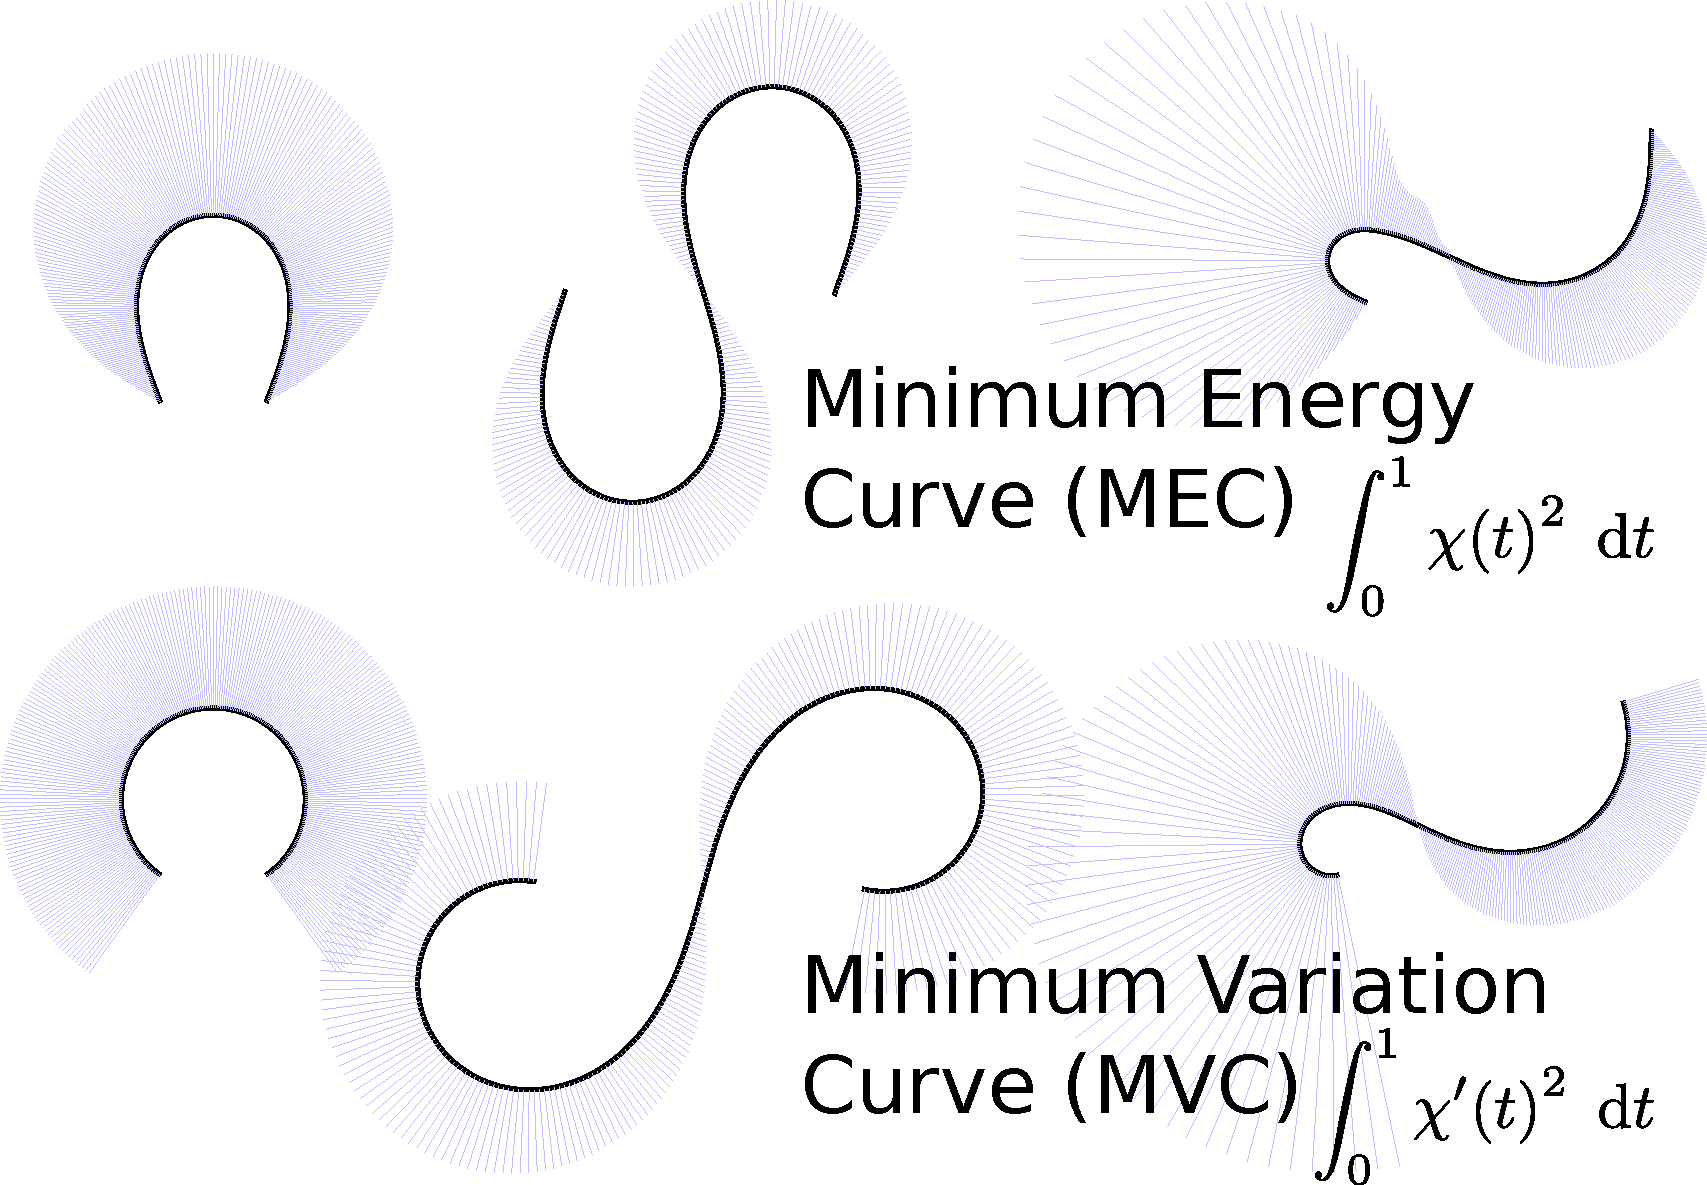
\includegraphics[width=\textwidth]{../resources/fairness_measures.pdf}}
			% MEC: derived from mechanical splines (steel band)
			% MEC always tries to have zero curvature at endpoints
			% generally: MVC tends to make curves with circular arcs/spirals, constant/linearly changing curvature
			% MEC doesn't work with curvature specifications
			% we choose MVC for our approach
		\end{frame}

		% B
		\begin{frame}
			\frametitle{Curve Derivation}
			\begin{itemize}
				\item turn descriptions into actual curves
				\item approach: nonlinear optimization on polynomial splines
				\begin{itemize}
					\item nonlinear optimization: flexible, allows for experimentation
					\item polynomial curves: simple, versatile
					\item polynomial splines: avoids polynomials of high degree
				\end{itemize}
			\end{itemize}
		\end{frame}

		% B
		\begin{frame}
			\frametitle{Optimization Problem}
			\begin{itemize}
				\item using
				\begin{itemize}
					\item objective function \(f : \function{\R{n}}{\RR}\)
					\item constraint function \(g : \function{\R{n}}{\R{m}}\)
					\item constraint bounds \(g_l, g_u \in \R{m}\)
				\end{itemize} 
				\item try to find an \(x^* \in \R{n}\) such that 
			\end{itemize}
			\begin{equation*}
				\begin{gathered}
					x^* = \argmin_{x \in \R{n}} \apply{f}{x}\\
					g_l \leq \apply{g}{x^*} \leq g_u
				\end{gathered}
			\end{equation*}
			% allows expressing soft optimization goals and hard constraints
			\begin{itemize}
				\item smooth optimization (interior point method)
			\end{itemize}
		\end{frame}

		% B 
		\begin{frame}
			\frametitle{Finding Curves as Optimization Problem}
			\begin{itemize}
				\item segment polynomials
			\end{itemize}
			\begin{equation*}
				\apply{\phi_i}{t} = \sum_j a_{i,j} \cdot t^j
			\end{equation*}
			\begin{itemize}
				\item segmentation
			\end{itemize}
			\center{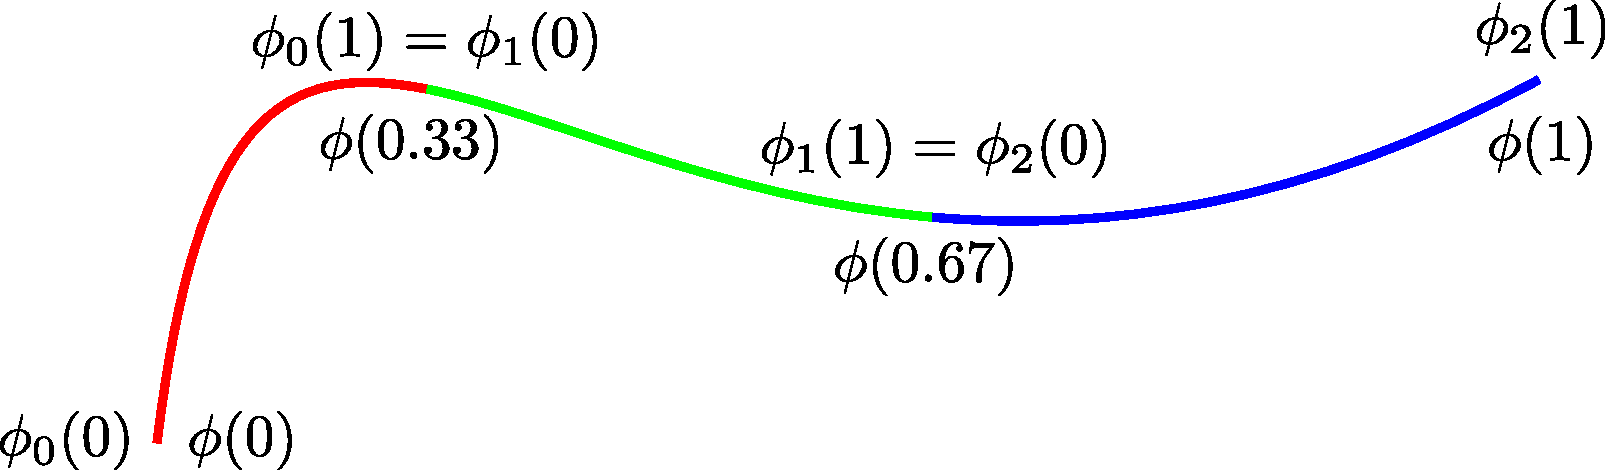
\includegraphics[width=\textwidth]{../resources/segmentation.pdf}}
			% these segments are invisible to the user, not related to the specification items
			\begin{itemize}
				\item optimization domain: coefficients \(a_{i,j}\)
			\end{itemize}
		\end{frame}

		% B
		\begin{frame}
			\frametitle{Covered Arc Length Function}
			\begin{itemize}
				\item \(\apply{\lambda}{t}\) relates parameter values to covered arc length
			\end{itemize}
			\center{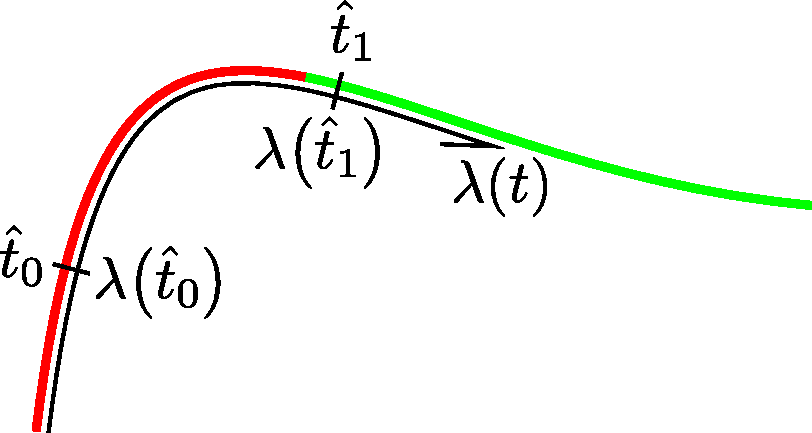
\includegraphics[width=50mm]{../resources/inverse_covered_arc_length.pdf}}
			\begin{itemize}
				% to state error terms for specifications with arc length positioning, the following has to be done
				\item example: find \(\hat{t}\), such that \(\apply{\lambda}{\hat{t}} = 0.4\) and \(\apply{\delta}{\hat{t}} = 15^\circ\)
				\item requires finding \(\apply{\lambda^{-1}}{\hat{t}}\)
				\item result determines segment for specification item
				% if it's \hat{t}_1, it's on the green segment
				\item error terms unsuitable for smooth optimization
				\item further complications: error terms for arc length and fairness measure
			\end{itemize}
		\end{frame}

		% B
		\begin{frame}
			\frametitle{Constant Speed}
			\begin{itemize}
				\item solution: add constant speed as optimization goal
				\item error term
			\end{itemize}
			\begin{equation*}
				\integral{0}{1}{\xp{\apply{\sigma}{t} - \hat{\lambda}}^2}{t}
			\end{equation*}
			\begin{itemize}
				\item covered arc length function approximately linear: \(\apply{\lambda}{t} \approx \hat{\lambda}t\)
				% makes inverse covered arc length function linear, too, 
				\item curve's total arc length approximately \(\hat{\lambda}\)
				\item error terms for specification items become trivial
			\end{itemize}
		\end{frame}

		% B
		\begin{frame}
			\frametitle{Continuity Connections}
			\begin{itemize}
				\item require \(\contg{2}\) continuity
				\item each segment is smooth, resulting spline may not be
				\item ensure \(\contg{2}\) continuity at segment connection points
				\item error terms
			\end{itemize}
			\begin{equation*}
				\begin{gathered}
					\apply{\phi_i}{1} - \apply{\phi_{i + 1}}{0}\\
					\apply{\phi'_i}{1} - \apply{\phi'_{i + 1}}{0}\\
					\apply{\phi''_i}{1} - \apply{\phi''_{i + 1}}{0}
				\end{gathered}
			\end{equation*}
			% constant speed collapses G2 and C2 continuity, requiring C2 continuity isn't asking too much
		\end{frame}

		% B
		\begin{frame}
			\frametitle{Fairness Error}
			\begin{itemize}
				\item MVC fairness measure
				\item error term
			\end{itemize}
			\begin{equation*}
				\integral{0}{1}{\apply{\chi'}{t}^2}{t}
			\end{equation*}
		\end{frame}

		% B
		\begin{frame}
			\frametitle{Overall Curve Derivation Process}
			\begin{itemize}
				\item construct optimization problem from error terms
				\item compute coefficients with optimization solver
				\item build result curve from coefficients
			\end{itemize}
		\end{frame}

	\section{Implementation}

		% A
		\begin{frame}
			\frametitle{Architecture}
			\begin{itemize}
				\item programming language: C\#
				\begin{itemize}
					% familiar, high level
					\item platform independent
					\item interfaces with native code
					\item UI frameworks available
				\end{itemize}
				\item libraries
				\begin{itemize}
					\item Ipopt: numeric nonlinear optimization
					\item CasADi: automatic differentiation of terms
					\item GTK\#: UI library
				\end{itemize}
			\end{itemize}
		\end{frame}

		% A
		\begin{frame}
			\frametitle{Subsystems}
			\begin{itemize}
				\item Kurve: UI prototype
				\item Kurve.Curves: optimization of curves
				\item Wrappers.Casadi and Wrappers.Casadi.Native: APIs for CasADi and Ipopt
			\end{itemize}
		\end{frame}

		% A
		\begin{frame}
			\frametitle{Optimization Steps}
			\center{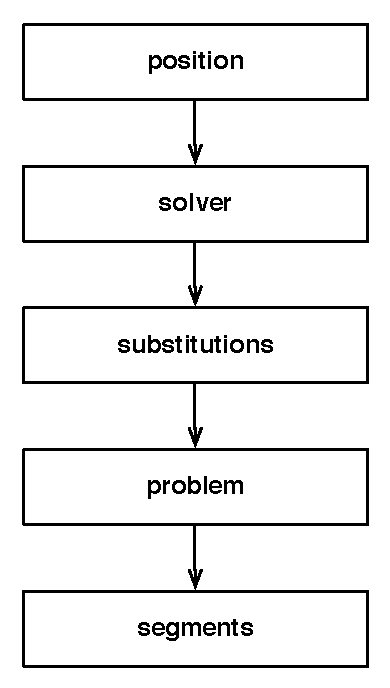
\includegraphics[width=35mm]{../resources/optimization_step_dag.pdf}}\\
		\end{frame}

	\section{Demo}

		% topics of the demo
		% 1. explain features
		%	- add curve
		% 	- increase length
		% 	- modify point specification
		% 	- change position of point
		% 	- toggle direction, demonstrate
		% 	- add specification in middle
		% 	- toggle curvature, decrease it
		%	- demonstrate length insertion (decrease right segment)
		% 	- increase segment count (now manages to do circle arcs now!)
		% 	- remove left P (PD -> D)
		% 	- rotate uniquely specificed arc
		% 	- instability: how to fix
		% 	- say that we have save load export
		% 2. example mane fluttershy: specifying curvature is awesome. compare with beziere
		% 	- load 2.xml. curvature specifications!
		% 3. circle arcs via arc length (fluttershy chin/mouth/ear
		% 	- reuse old winow. add arc at ear
		% 5. euler spiral (we're doing it LIVE!
		% 	- new window, create it. symmetric.
		% 7. many local potentially shitty optima, can be fixed by stretching/dragging etc.
		% 	- load 7.xml; remove by dragging..
		% 8. Problem: slow.  May converge slowly or not at all
		% 	- load 8.xml
		% 10. Pathological local minima
		% 	- 10.xml
		% 11. Requests please.
		% 

		\begin{frame}
			\frametitle{Demo}
		\end{frame}

	\section{Conclusion}

		% B
		\begin{frame}
			\frametitle{Conclusion}
			\begin{itemize}
				\item description-based curves look promising
				\item most problems of prototype caused by optimization
				% optimization approach will not be pursued further, even though performance could be improved some more
				\item future work
				\begin{itemize}
					\item research more constructive approach for building curves
					\item add even more expressiveness to description language
					% for instance making specification of arc length optional
					\item more research on soft specifications
					\item usability study with actual designers
					\item Inkscape integration
				\end{itemize}
			\end{itemize}
		\end{frame}

\end{document}
